\section{Theoretical Analysis}
\label{sec:analysis}
First of all, we performed an operating point analysis in order to check if the transistor was operating in the forward active region.
\begin{table}[h!]
  \centering
  \begin{tabular}{|l|r|}
    \hline    
    {\bf Name} & {\bf Values} \\ \hline
    \input{th_data_tab} 
  \end{tabular}
  \caption{Operating point analysis results.}
  \label{tab:data}
\end{table}

As we can see, VCE is greater than VBEON (0.7V), so we're good to go.
\subsection{Gain Stage}
For the gain stage, the analysis of the incremental circuit yielded the following results:
\begin{table}[h]
  \centering
  \begin{tabular}{|l|r|}
    \hline    
    {\bf Name} & {\bf Values} \\ \hline
    \input{gain_tab} 
  \end{tabular}
  \caption{Gain stage theoretical results}
  \label{tab:gain}
\end{table}

We can clearly see the need for an output stage, given the magnitude of the output impedance. The gain is also significant, and we'll strive for a unitary gain in the output stage in order not to sacrifice this.

\subsection{Output Stage}
As before, we perform a DC operating point analysis:
\begin{table}[h!]
  \centering
  \begin{tabular}{|l|r|}
    \hline    
    {\bf Name} & {\bf Values} \\ \hline
    \input{outoper_tab} 
  \end{tabular}
  \caption{Operating point analysis results.}
  \label{tab:data2}
\end{table}
From both the table and the following equation we can understand that the voltage drop in this transistor is greater than 0.7V and so it is operating in the forward active region.
\begin{equation}
\label{eqn:collector}
V_{emit2}=V_{coll}+V_{EBON};
\end{equation}

Next, we present the results of the output stage theoretical model.
\begin{table}[h]
  \centering
  \begin{tabular}{|l|r|}
    \hline    
    {\bf Name} & {\bf Values} \\ \hline
    \input{output_tab} 
  \end{tabular}
  \caption{Output stage theoretical results}
  \label{tab:output}
\end{table}
\pagebreak

As desired, the input impedance of this stage is more than 10 times greater than the output impedance of the gain stage. This means that the circuit experiences little signal loss. As well, the output impedance of this stage is desirably low when compared to the 8 Ohm of the speakers.
At last, the total circuit gain results.

\begin{table}[h]
  \centering
  \begin{tabular}{|l|r|}
    \hline    
    {\bf Name} & {\bf Values} \\ \hline
    \input{circuit_tab} 
  \end{tabular}
  \caption{Total circuit theoretical gain results}
  \label{tab:output}
\end{table}
The gain is slightly lower than the product of the two previous gains, likely due to some signal loss in the interface between stages.
Besides this approach, we plotted the frequency response of the circuit for the output voltage of the circuit, in terms of gain and phase difference:

\begin{figure}[!h] \centering
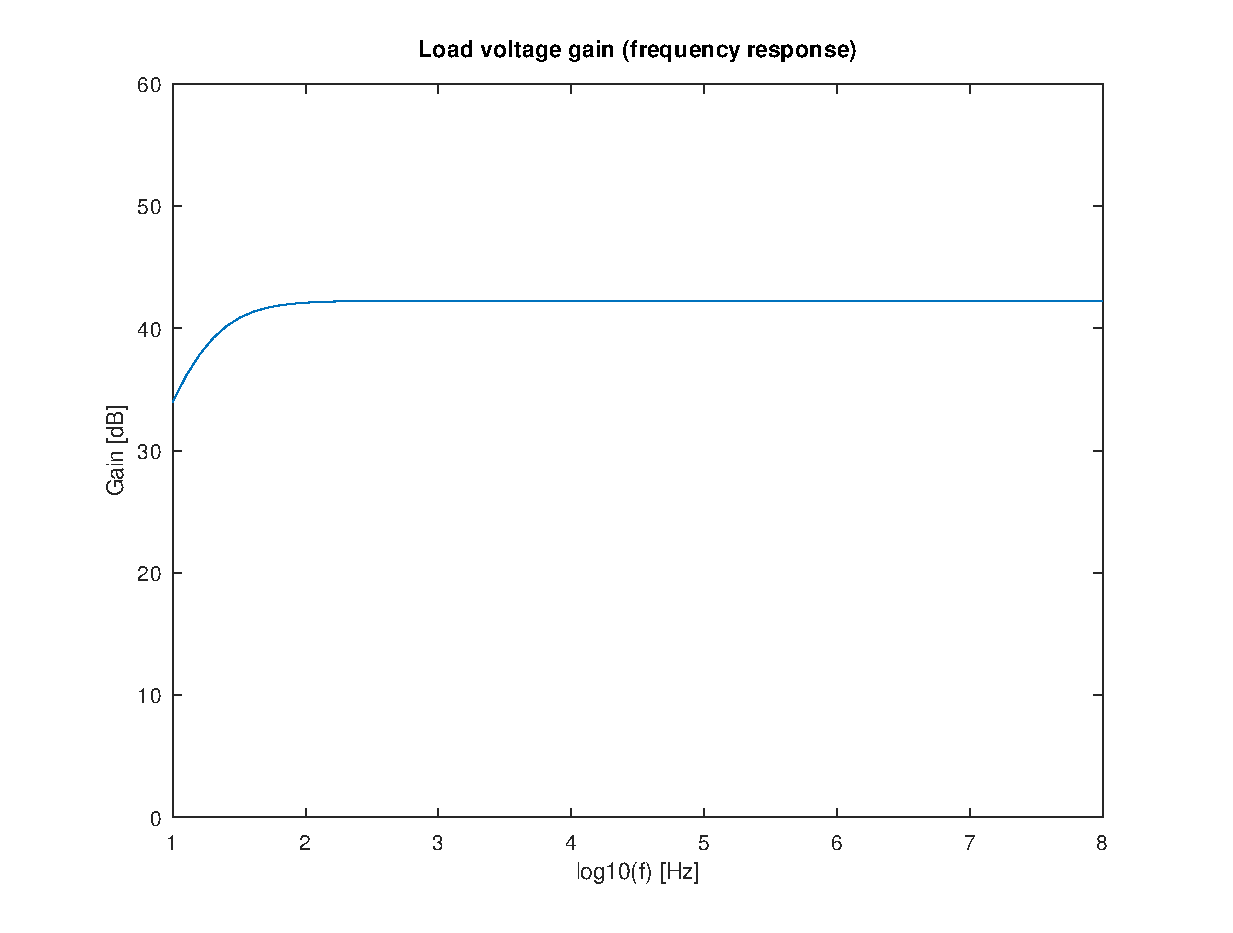
\includegraphics[width=0.6\linewidth]{Gain.eps}
\caption{Load output voltage gain (frequency response).}
\label{fig:gainfreq}
\end{figure}

\begin{figure}[!h] \centering
\includegraphics[width=0.6\linewidth]{Phase.eps}
\caption{Load output voltage phase difference (frequency response).}
\label{fig:phasefreq}
\end{figure}

\pagebreak

For the medium frequencies (within the bandwidth) we obtained the following gain figure.

We also determined the lower cut-off frequency, which yielded close to 20 Hz, the lowest frequency the human ear can perceive as a musical note. This was achieved by finding the point on the gain frequency response plot that had a 3 decibel drop relative to the maximum gain.
\begin{table}[h]
  \centering
  \begin{tabular}{|l|r|}
    \hline    
    {\bf Name} & {\bf Values} \\ \hline
    \input{frequency_tab} 
  \end{tabular}
  \caption{Gain for medium frequencies and lower cut-off frequency of the output voltage signal.}
  \label{tab:freq}
\end{table}
